% Software Framework %
\chapter{Software Framework}
\label{chapter2}
Automatic analysis and modification of program code is a widely applied technique to quickly optimize and customize many complex programs at once. \CLANG provides a library that makes it possible to write tools that can be used primarily for \SOUTOSOU transformation of \C, \CPP, and \OC programs~\cite{ClangLibTooling}. This interface enables the developer to use the powerful \astsmall and the extensively developed infrastructure of \CLANG. For example, Fabian Schlebush et al.~\cite{schlebushrelwork} used the infrastructure to categorize high performance computation applications. Another example is the approach of Alexander Hück et al.~\cite{hueckrelwork} to rewrite incompatible code resulting from upgrading to newer versions into error free code. In order to develop a tool that is suitable for wrapping \roismall with performance counters, we will also use the \LLVM compiler infrastructure and the front-end framework \CLANG that is built on top of it. The former is a modern compiler architecture that contains a variety of tools and libraries to optimize high-level languages, like \CPP, during translation into machine code~\cite{LLVMPaper}. \CLANG allows to analyze, structure and check the code for semantic and syntactic errors~\cite{ClangLanding}. Furthermore, the front-end part of the compiler is capable of transforming the program code into an \astsmall, which can then be translated into machine language by the back-end. Especially the front-end part is interesting for our type of application, as the transformation from \SOUTOSOU is supported by predefined macro functions that combine a large number of individual instructions. This chapter explains the fundamental concepts behind the software framework and focuses on the \astsmall of \CPP applications created by \CLANG.

\section{The LLVM Compiler Infrastructure}
The back-end part of the compiler is responsible for transforming the provided syntax tree into machine code. To achieve this, \LLVM creates the so-called \LLVM \emph{intermediate representation}. This is an intermediate machine code that can be used to abstract different programming languages. This code can now be used to apply optimization methods independently of the input language. After all optimizations have been completed, the intermediate code can be compiled into machine code, again with the possibility of addressing different processor architectures and thus being target-independent~\cite{LLVMInformation}. However, as the \LLVM project has grown, several sub-projects have been added, one of which is the \CLANG front-end framework. This project deals with the fast and efficient compilation of \C, \CPP, and \OC applications~\cite{LLVMLanding}. 

\section{Clang Language Frontend for LLVM}
\CLANG is a front-end framework for \LLVM that is capable of translating programming languages from the \C family and also provides an infrastructure for the development of tools~\cite{ClangLanding}. As a front-end part of a compiler architecture, one of the most fundamental tasks is the creation of an \astsmall. In general, an \astsmall is a generalized representation of the written programming language, where a node represents an instruction. To create such a model, the given source code must be analyzed and checked for errors so that it can finally be represented in a structured way. 

In \CLANG, these nodes do not contain any information about dependencies, which makes the system very optimized in terms of memory consumption and speed. The data about the connections between the nodes and the general structure of the program is stored in the so-called \IDTAB~\cite{ClangASTVideo,ClangASTVideoNachweis}. In order for the user to navigate through the model, an \ENTPOI is needed, which in \CLANG is called \lstinline{ASTContext} and can be reached by using the function \lstinline{getTranslationUnitDecl()}. This top level node contains the \IDTAB, which allows the user to navigate to the single nodes using pointers. Furthermore, the different nodes in \CLANG are only divided into three large classes, \declssmall, \STATS, and types, whereby each powerful core class contains a large subset of different sub-classes~\cite{ClangAST}. For instance, there is a large number of different types of \declssmall that are all grouped under the super-class \declssmall. The best known and most commonly used is the \DECL of a variable. To give another example, \COMSTMTS and \BINOPT are grouped under the super-class \STATS. It should also be noted that there is no general superclass for all types of nodes, but that all nodes are assigned to one of the core classes. Since each core class has a different type of navigation, there is no possibility to visit all nodes equally. For instance, we can navigate through an \lstinline{if}-\STAT by calling the functions \lstinline{getThat()} or \lstinline{getElse()}. In contrast, the function \lstinline{getBody()} must be called to access the contents of a \lstinline{while}- or a \lstinline{for}-loop.

Figure~\ref{fig:intro:dump ast example} shows the \astsmall of the simple \CPP program we introduced in Listing~\ref{lst:intro:example}. The representation of the \astsmall can be displayed by executing the command \lstinline{clang-check -ast-dump [Filename]}~\cite{ClangCheck}. It can be seen that the topmost instance of the tree is represented by the node \lstinline{TralsationUnitDecl}. In the first sub-level, we find the nodes of type \lstinline{TypedefDecl}, which describe predefined types like integer or strings. Furthermore, \declssmall of functions are shown at this level. The node \lstinline{CompoundStmt} groups all \STATS and expressions that are children of another node. If we look at the lower levels of the tree, we finally see the individual \STATS that are each represented by a node. If we take a closer look at the information provided for each node, the start location and the end location can be noted. The data about the location is stored in the so-called \SOUMNG, each pointing to a token in the programming code. To get these locations in a \CLANG application, the functions \lstinline{getLocStart()} or \lstinline{getLocEnd()}, which point to the first or the last token of the instruction, can be executed. 

\begin{figure}[t]
  \centering
  \caption{An Example of the \AST Provided by \CLANG.} 
  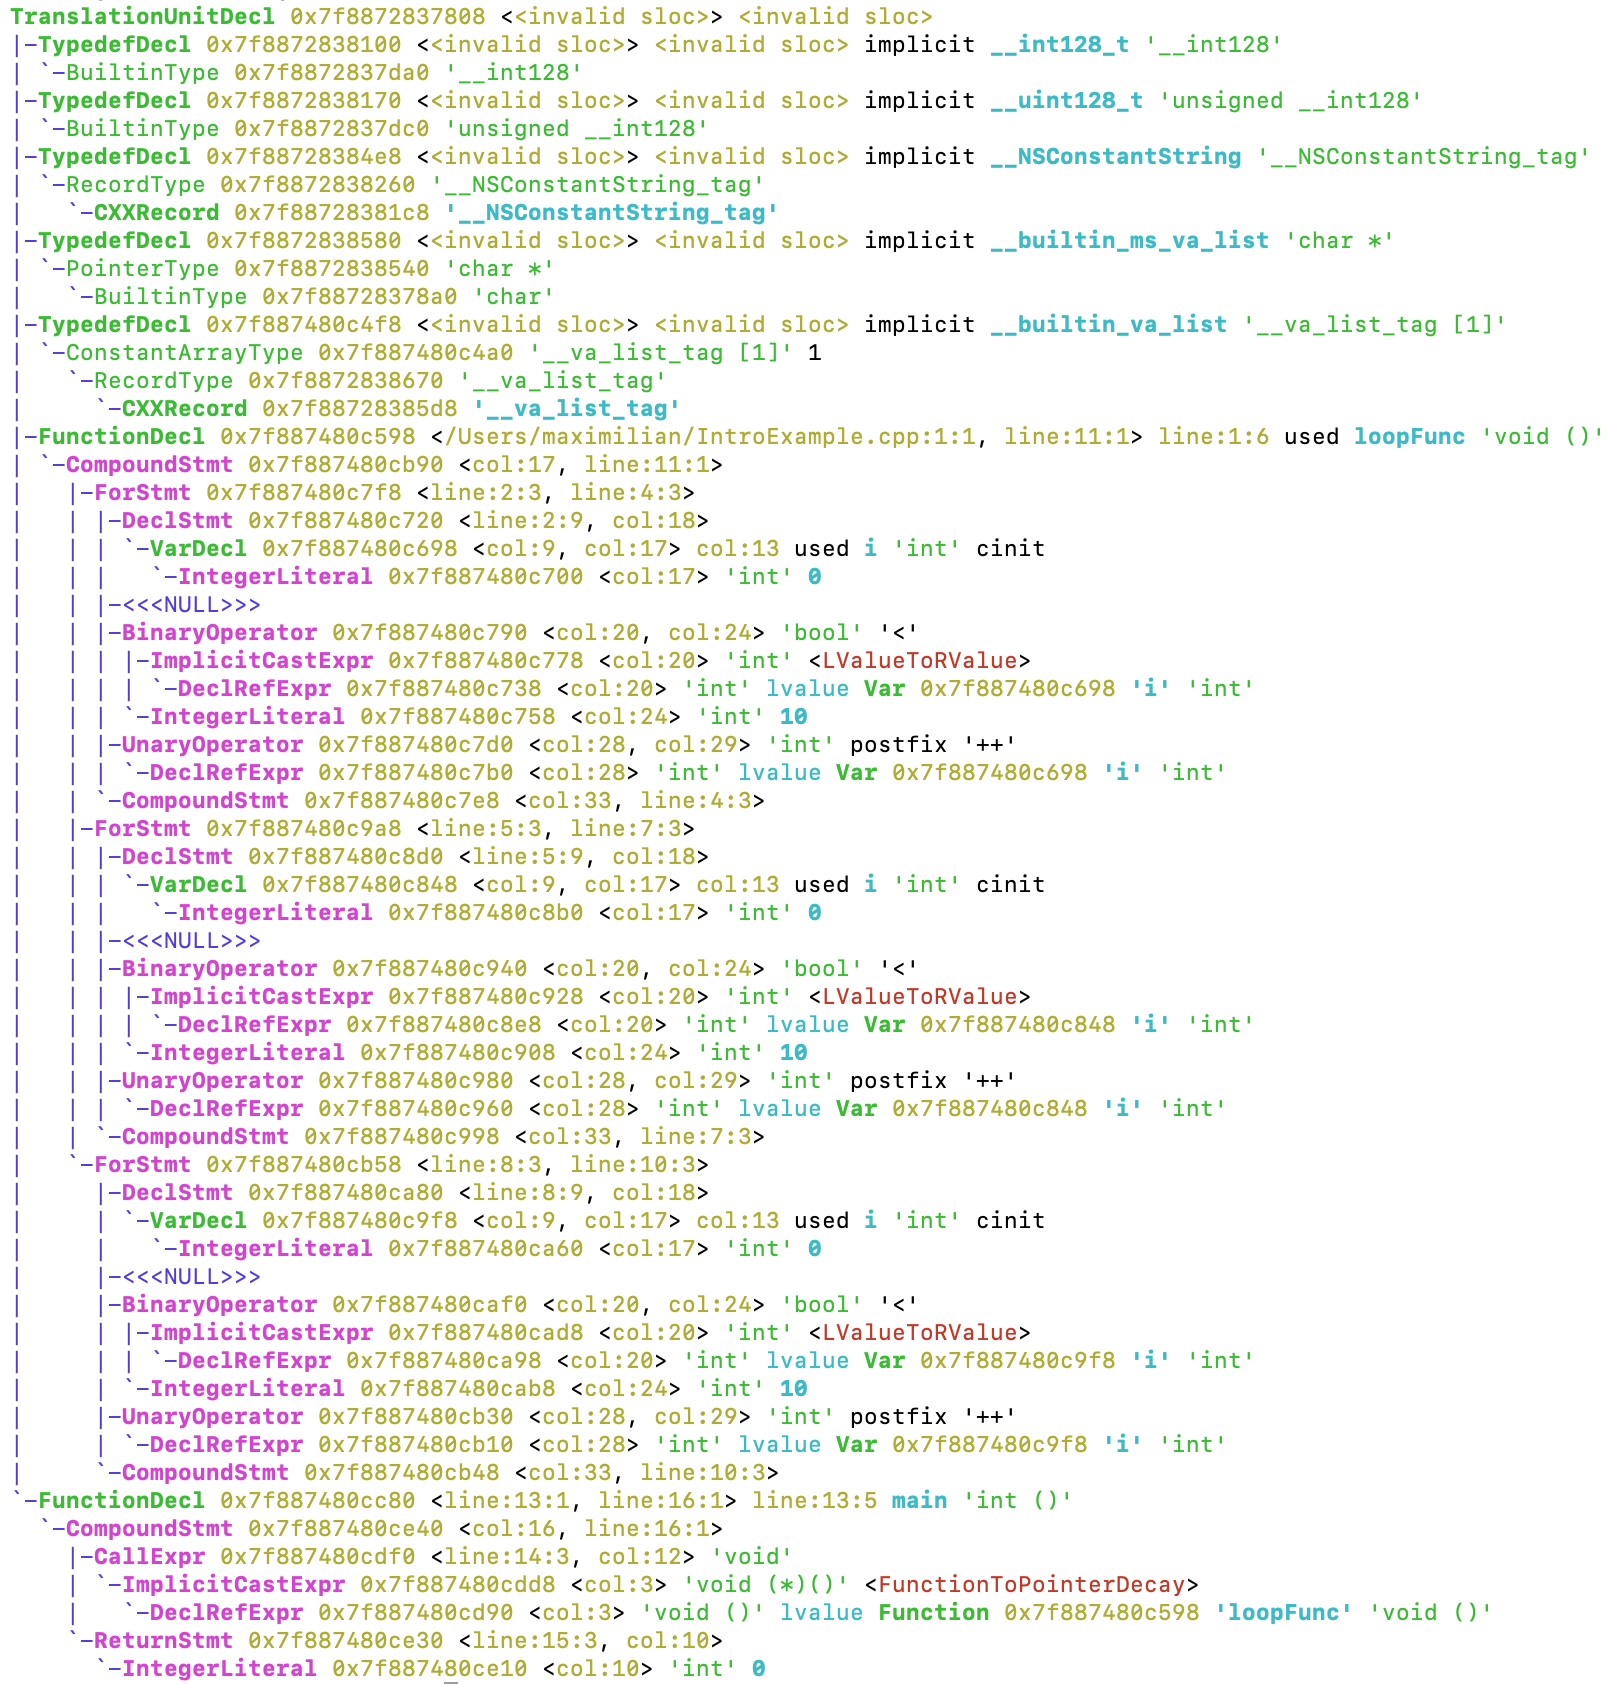
\includegraphics[width=1\textwidth]{graphics/t_ast.png}
  \label{fig:intro:dump ast example}
\end{figure}

To enable the user to develop his own tool based on the \CLANG framework, the so-called \lstinline{RecursiveASTVisitor} is provided. This contains a set of predefined functions and brings together all the information on how to access different \declssmall, \STATS and types. For instance, the method \lstinline{VisiteStmt(void)} provides a routine to traverse all the \STATS in the code. Users can access these interfaces to implement their own logic and perform \SOUTOSOU transformations. \CLANG's functions and existing infrastructure can thus be used to find places in an application and insert the desired code there~\cite{ClangLibTooling}. Therefore, the framework is very well-suited for writing an application that satisfies the objectives of the thesis. For the development of the tool we will use \LLVM version 14.0.1 and \CLANG version 14.0.1 built on top of it, also relying on the associated documentation~\cite{ClangDocs}. 